\section*{Diagramas de Minkowski}
\begin{align*}
    &1. \text{ Cono de luz: } x=\pm ct \;\; (---)\\
    &2. \text{ Evento $E$ en espaciotiempo representado por punto $(x,ct)$, denotado como $(ct,x)$.}\\
    &3. \text{ Línea de mundo de observador en reposo: } x=0.\\
    &4. \text{ Línea de mundo observador moviéndose a velocidad $v$: } x=vt.\\
    &5. \text{ Ejes sistema movido: } ct': x= vt \;x': ct=\tfrac{v}{c}x \; \text{ (simétricos respecto rayo de luz)} \\
    &6. \text{ Hipérbola invariante: }
    \left |
    \begin{array}{l}
    \textcolor{lightgray}{\rule{0.5em}{0,5em}}\; c^2t^2- x^2 = 1\; \text{ (intersección marca unidades en $ct'$)}\\
    \textcolor{gray}{\rule{0.5em}{0,5em}}\; x^2-c^2t^2 = 1\; \text{ (intersección marca unidades en $x$)}  
\end{array}
\right. \\
    &7. \text{ Para medir }
     \left|
\begin{array}{l}
\text{tiempo ($ct'$})\rightarrow \text{proyecta hacia el eje $ct'$ siguiendo paralela a $x'$} \\
\text{posición ($x$)} \rightarrow \text{proyecta hacia el eje $x'$ siguiendo paralela a $ct'$}
\end{array}
\right. \\
&8. \text{ Cambio base entre sistemas inerciales: } e_{0'}=\gamma (e_0 + \beta e_1) \; \; \; e_{1'}=\gamma(e_1+ \beta e_0)
\end{align*}
\vspace{3pt}
$\;\;\;\;\;\;\; x^0 \equiv ct, \; x^1 \equiv x, \; \gamma =\frac{1}{\sqrt{1-\beta^2}}, \;  \beta=\frac{v}{c}, \;  g_{\scalebox{0.8}{Minkowski}}=g^{-1}=\text{diag}(-1,1)\Rightarrow\Gamma^\alpha_{\beta \sigma} = 0$

\begin{minipage}{0.48\linewidth}
    \centering
\begin{tikzpicture}[scale=0.75,>=stealth]
  %===== Parámetros =====
  \pgfmathsetmacro{\v}{0.6}        % velocidad (c=1)
  \pgfmathsetmacro{\g}{1/sqrt(1-\v*\v)} % gamma
  \pgfmathsetmacro{\X}{2.5}         % semiancho de la ventana

  %===== Ejes t y x =====
  \draw[->] (-\X,0) -- (\X,0) node[right] {$x$};
  \draw[->] (0,-\X) -- (0,\X) node[above] {$ct$};
  \node[yshift=-4pt, xshift=-10pt] at (0,0) {\scriptsize{$O$}};

  %===== Líneas de luz =====
  \draw[dashed] (-\X,-\X) -- (\X,\X);
  \draw[dashed] (-\X,\X) -- (\X,-\X);

  %===== Ejes primados (marco movido) =====
  % t' : x = v t  =>  t = (1/v) x  (pendiente 1/v en el plano (x,t))
  % x' : t = v x  (pendiente v)
  \path[name path=tprime] (0,0) -- ({\v*\X},{\X});
  \path[name path=xprime] (0,0) -- ({\X},{\v*\X});
  \draw[red,->,name path global/.expanded=tprime] (0,0) -- ({\v*\X},{\X}) node[above right] {$ct'$};
  \draw[red,->,name path global/.expanded=xprime] (0,0) -- ({\X},{\v*\X}) node[above] {$x'$};

  %===== Hipérbola invariante t^2 - x^2 = 1 =====
  \draw[lightgray,domain=-\X:\X,smooth,variable=\x] plot (\x,{sqrt(\x*\x+1)});
  \draw[lightgray,domain=-\X:\X,smooth,variable=\x] plot (\x,{-sqrt(\x*\x+1)});

  % Hipérbola x^2 - t^2 = 1 (espacio)
\draw[gray,domain=1:\X,smooth,variable=\x] plot (\x,{sqrt(\x*\x-1)});
\draw[gray,domain=1:\X,smooth,variable=\x] plot (\x,{-sqrt(\x*\x-1)});
\draw[gray,domain=-\X:-1,smooth,variable=\x] plot (\x,{sqrt(\x*\x-1)});
\draw[gray,domain=-\X:-1,smooth,variable=\x] plot (\x,{-sqrt(\x*\x-1)});

  %===== Unidades sobre ejes primados por intersección con la hipérbola =====
  % En t': (x,t) = (gamma*v, gamma)
  % En x': (x,t) = (gamma, gamma*v)
  \fill[red] ({\g*\v},{\g}) circle (0.7pt);
  \fill[red] ({\g},{\g*\v}) circle (0.7pt);

  %===== Evento de ejemplo =====
  \coordinate (E) at (1,2); % (x,t) = (1,2)
  \filldraw[blue] (E) circle (1pt) node[ above left] {$E$};

  %===== Guías paralelas a x' y t' que pasan por E =====
  % Paralela a x' (pendiente v)
  \path[name path=gxprimeA] ($(E)+(1,-1*\v)$) -- ($(E)+(1,1*\v)$);
  \draw[blue!50,dashed,name path global/.expanded=gxprimeA] ($(E)+(-2,-2*\v)$) -- ($(E)+(2,2*\v)$)
    node[near end,sloped, xshift=19pt,
    yshift=4pt] {$\parallel\,x'$};

  % Paralela a t' (pendiente 1/v)
  \path[name path=gtprimeA] ($(E)+(-1,{-1/\v})$) -- ($(E)+(1,{1/\v})$);
  \draw[blue!50,dashed,name path global/.expanded=gtprimeA] ($(E)+(-1,{-1/\v})$) -- ($(E)+(1,{1/\v})$)
    node[near end,sloped,xshift=11pt, yshift=4pt] {$\parallel\,ct'$};

  %===== Intersecciones para proyecciones (lectura de t' y x') =====
  \path[name intersections={of=gxprimeA and tprime,by=Itp}];   % guía || x' con eje t'
  \path[name intersections={of=gtprimeA and xprime,by=Ixp}];  % guía || t' con eje x'



  %===== Marcas visuales opcionales en ejes primados =====
  \draw[red] ({0.5*\v*\X},{0.5*\X}) -- ++({0.06},{-0.06/\v});  % pequeña marca en t'
  \draw[red] ({0.5*\X},{0.5*\v*\X}) -- ++({-0.06*\v},{0.06});  % pequeña marca en x'

\end{tikzpicture}
\vspace{-10pt}
    \hyphenpenalty=10000
    \exhyphenpenalty=10000
    \captionof*{figure}{\tiny Diagrama de Minkowski con dos sistemas de coordenadas: observador en reposo $\textcolor{black}{\rule{0.5em}{0,5em}}$ y observador en movimiento $\textcolor{red}{\rule{0.5em}{0,5em}}$.}
\end{minipage}
\hfill
\begin{minipage}{0.48\linewidth}
    \centering
    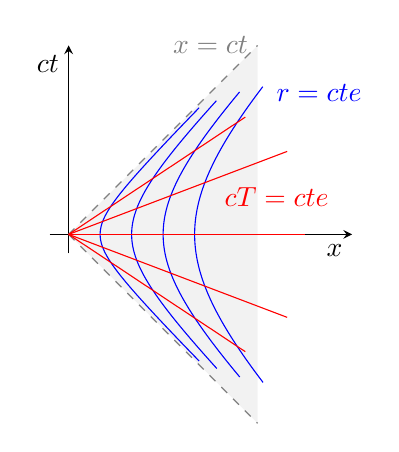
\begin{tikzpicture}[scale=1.2,>=stealth]

% Cuña de Rindler
\fill[gray!10] (0,0) -- (2,2) -- (2,-2) -- cycle;

% Ejes
\draw[->] (-0.2,0) -- (3,0) node[below left] {$x$};
\draw[->] (0,-0.2) -- (0,2) node[below left] {$ct$};

% Cono de luz
\draw[dashed, gray] (0,0) -- (2,2) node[above,left] {$x=ct$};
\draw[dashed, gray] (0,0) -- (2,-2);



% Hipérbolas: xi = const
\foreach \xi in {1/3}{
    \draw[blue, domain=-2.1:2.1, samples=200, variable=\eta] 
        plot ({\xi*cosh(\eta)}, {\xi*sinh(\eta)});
}

% Hipérbolas: xi = const
\foreach \xi in {2/3}{
    \draw[blue, domain=-1.5:1.5, samples=200, variable=\eta] 
        plot ({\xi*cosh(\eta)}, {\xi*sinh(\eta)});
}

\foreach \xi in {3/3}{
    \draw[blue, domain=-1.2:1.2, samples=200, variable=\eta] 
        plot ({\xi*cosh(\eta)}, {\xi*sinh(\eta)});
}

\foreach \xi in {4/3}{
    \draw[blue, domain=-1:1, samples=200, variable=\eta] 
        plot ({\xi*cosh(\eta)}, {\xi*sinh(\eta)});
}

% Rectas eta = const (líneas de simultaneidad)
\foreach \eta in {-0.8,-0.4,0,0.4,0.8}{
    \pgfmathsetmacro{\m}{tanh(\eta)}
    \draw[red] (0,0) -- ({2.5/cosh(\eta)}, {2.5*tanh(\eta)/cosh(\eta)});
}

% Etiquetas
\node[blue] at (2.65,1.5) {$r = \text{cte}$};
\node[red] at (2.2,0.4) {$cT = \text{cte}$};

\end{tikzpicture}
 \hyphenpenalty=10000
    \exhyphenpenalty=10000
    \captionof*{figure}{\tiny Coordenadas de Rindler en el espacio-tiempo de Minkowski. \textcolor{blue}{Hipérbolas}: observador uniformemente acelerado. \textcolor{red}{Líneas}: instantes simultáneos en su marco.}
\end{minipage}





